\subsection{Accounting for generalization through group adjustments improves DRO}\label{sec:experiments_adjustments}
In the previous section, we optimized for the worst-group \emph{training} loss via DRO \refeqn{htdro}, relying on regularization to control the worst-group generalization gap and
translate good worst-group training loss to good worst-group test loss.
However, even with regularization, the generalization gap can vary significantly across groups: in the Waterbirds DRO model with a strong $\Ltwo$ penalty, the smallest group has a train-test accuracy gap of $15.4\%$ compared to just $1.0\%$ for the largest group.
This suggests that we can obtain better worst-group test loss if at training time, we prioritize obtaining lower training loss on the groups that we expect to have a larger generalization gap.

We make this approach concrete by directly minimizing an estimated upper bound on the worst-group test loss,
inspired by ideas from structural risk minimization \citep{vapnik1992principles}.
The key consideration is that each group $g$ has its own generalization gap $\gengap = \E_{(x,y) \sim P_g}[\ell(\theta; (x,y))] - \E_{(x,y) \sim \hP_g}[\ell(\theta; (x,y))]$.
To approximate optimizing for the worst-group test loss
$\sR(\theta) = \max_{g \in \sG} \E_{(x,y) \sim \hP_g}[\ell(\theta; (x,y))] + \gengap$,
we propose using the simple, parameter-independent heuristic $\hatgengap = C/\sqrt{n_g}$,
where $n_g$ is the group size for $g$ and $C$ is a model capacity constant which we treat as a hyperparameter. This gives the \emph{group-adjusted} DRO estimator
\begin{align}\label{eqn:htadj}
    \htadj \eqdef \argmin_{\theta \in \Theta} \ \underset{g \in \sG}{\vphantom{\argmin}\max} \ \left\{ \E_{(x, y) \sim \hP_g}[\ell(\theta; (x, y))] + \frac{C}{\sqrt{n_g}}\right\}.
\end{align}
The scaling with $1 / \sqrt{n_g}$ reflects how smaller groups are more prone to overfitting
than larger groups, and is inspired by the general size dependence of model-complexity-based generalization bounds (see, e.g., \citet{cao2019learning}).

By incorporating group adjustments in \refeqn{htadj},
we encourage the model to focus more on fitting the smaller groups.
We note that this method of using a $1/\sqrt{n}$ surrogate for the generalization gap only works in the group DRO setting, where we consider the worst-group loss over groups of different sizes. It does not apply in the ERM setting; if we were minimizing average training loss, the $1/\sqrt{n}$ term would simply be a constant and not affect the optimization.


\paragraph{Results.} We evaluate group adjustments using group DRO models with strong $\Ltwo$ penalties (as in \refsec{experiments_complexity_control}). In Waterbirds ($\lambda=1.0$), worst-group test accuracy improves by $5.9\%$, cutting the error rate by more than a third (\reftab{adj} and \reffig{adj}). The improvements in CelebA ($\lambda=0.1$) are more modest, with worst-group accuracy increasing by $1.1\%$; $\Ltwo$ penalties are more effective in CelebA and there is not as much variation in the generalization gaps by group at $\lambda=0.1$.
We did not evaluate group adjustments on MultiNLI as it did not benefit from stronger $\Ltwo$ penalties.

Empirically, group adjustments also help in the early stopping setting of \refsec{experiments_complexity_control} (in the next section,
we evaluate models with group adjustments and early stopping across a grid of $\Ltwo$ penalty strengths). However, it is difficult to rigorously study the effects of early stopping (e.g., because the group losses have not converged to a stable value), so we leave a more thorough investigation of the interaction between early stopping and group adjustments to future work.

\begin{table}
  \vspace{-5mm}
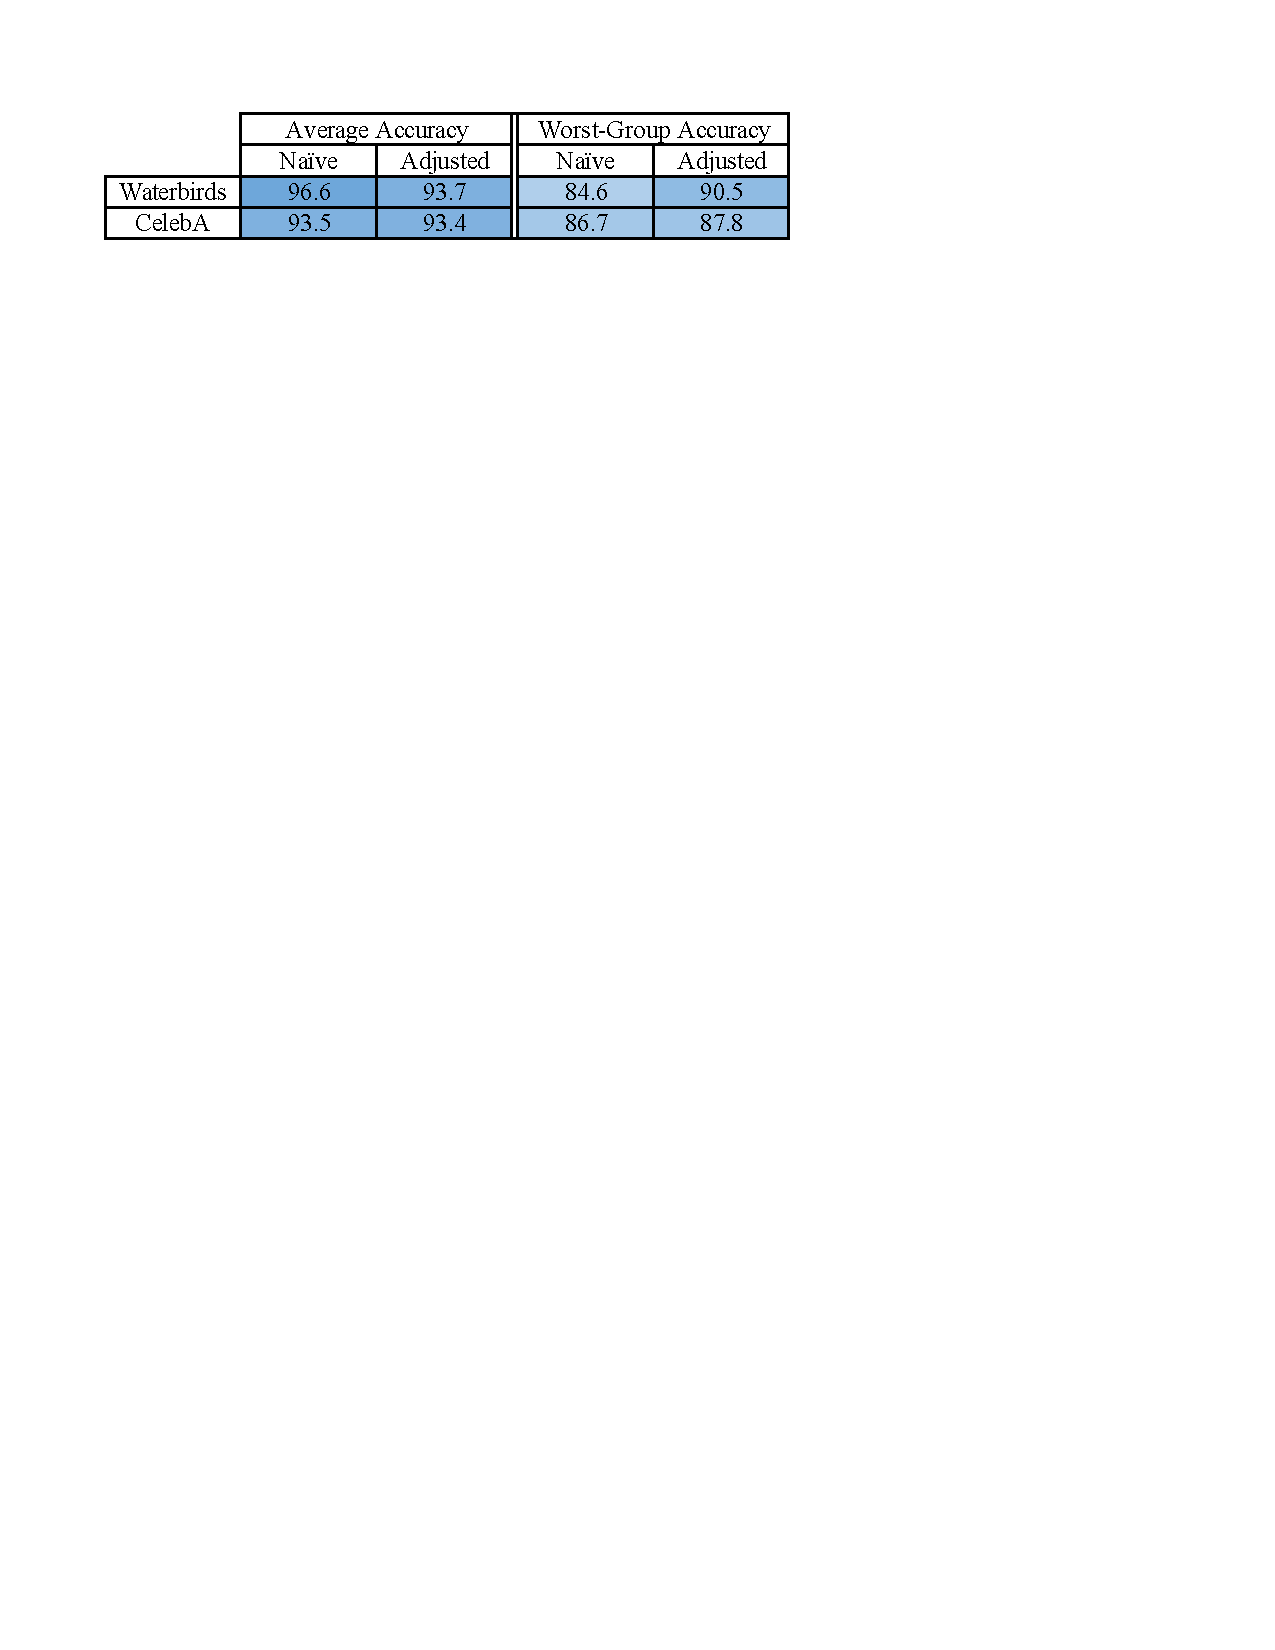
\includegraphics[width=0.6\textwidth]{figs/table_2.pdf}
\caption{Average and worst-group test accuracies with and without group adjustments. Group adjustments improve worst-group accuracy, though average accuracy drops for Waterbirds.}
\label{tab:adj}
\end{table}

\begin{figure}
  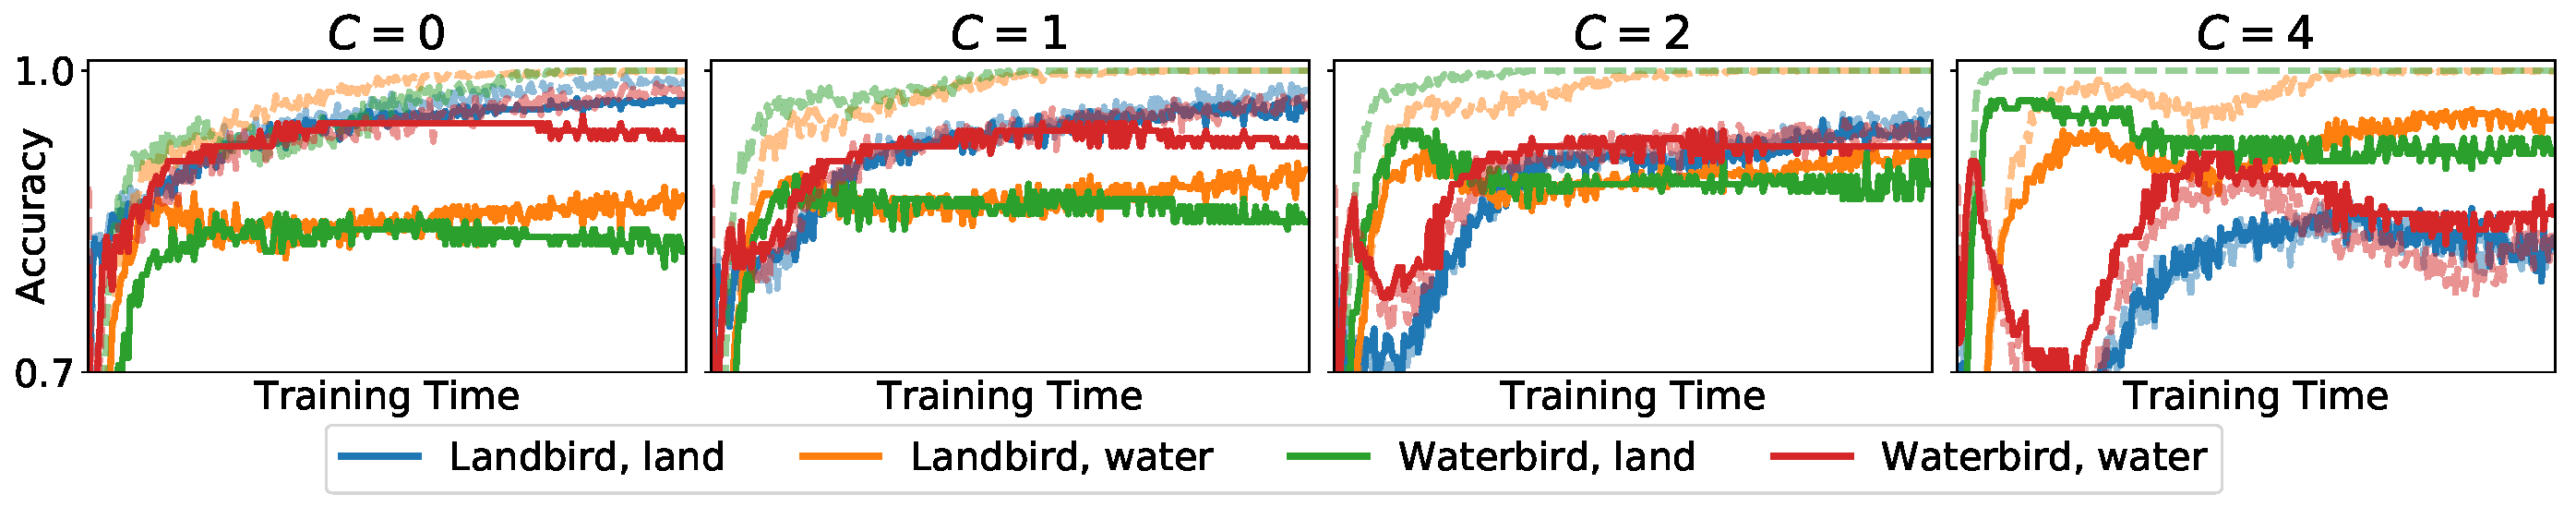
\includegraphics[width=\textwidth]{figs/group_adj_waterbirds.pdf}
  \caption{
    Training (light) and validation (dark) accuracies for each group over time,
    for different adjustments $C$.
    When $C=0$, the generalization gap for waterbirds on land (green line) is large, dragging down worst-group accuracy.
    At $C=2$, which has the best worst-group validation accuracy, the accuracies are balanced.
    At $C=4$, we overcompensate for group sizes, so smaller groups (e.g., waterbirds on land) do better at the expense of larger groups (e.g., landbirds on land).
}
\label{fig:adj}
\end{figure}
